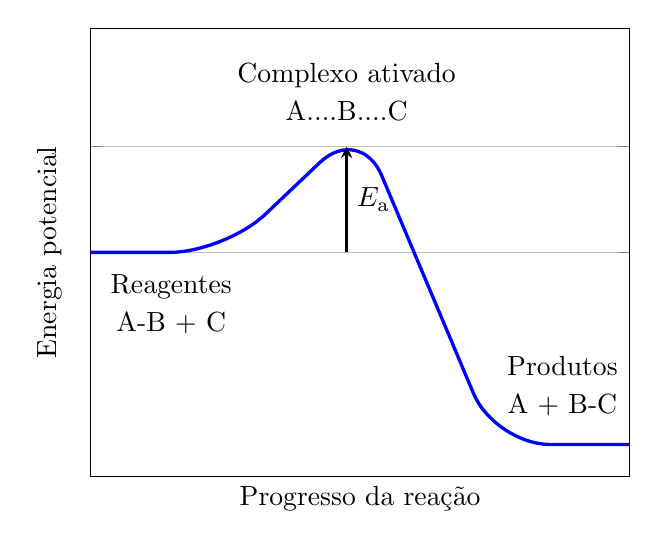
\begin{tikzpicture}
    \begin{axis}
        [
            grid = major,
            ylabel = {Energia potencial},
            xlabel = {Progresso da reação},
            xmin = 0, xmax = 4,
            ymin = -0.5, ymax = 6.5,
            xtick = \empty,
            ytick = {3, 4.65},
            yticklabels = {},
        ]

        \draw [draw=blue, very thick, rounded corners=2em]
            (axis cs: 0, 3) -- 
            (axis cs: 1, 3) -- 
            (axis cs: 2, 5) -- 
            (axis cs: 3, 0) --
            (axis cs: 4, 0);

        \node [ below, align=center ] at (axis cs:0.6,2.8) 
            { Reagentes \\[0.4ex] \ce{ A\bond{-}B + C } };
    
        \node [ above, align=center ] at (axis cs:1.9,4.9) 
            { Complexo ativado \\[0.4ex] \ce{ A\bond{....}B\bond{....}C } };

        \node [ above, align=center ] at (axis cs:3.5,0.3) 
            { Produtos \\[0.4ex] \ce{ A + B\bond{-}C } };

        \draw [ draw=black, thick, -stealth ]
            (axis cs: 1.9, 3.0) -- node [right] {$E_\mathrm{a}$}
            (axis cs: 1.9, 4.65);

     \end{axis}
 \end{tikzpicture}